% Main chapter 3:
% Inverse classification using generative models
\chapter{Inverse Classification using Generative Models}
\label{chap:ICGM}

The main innovation of this paper is inverse classification using generative models. This means to first train a generative model to learn to generate sequences. In the second step this model is then used to inversely classify data by generating sequences with an input vector. The sequences are then compared to the target and the input vector is iteratively adapted through gradient based methods. A more detailed explanation of the two step process can be found in the following two sections.

\section{Sequence Generation}

A recurrent neural network with LSTMs is trained to generate sequences from class inputs. The classes are represented as one-hot vectors, i.e. vectors where one entry is one and all others are zero. The model gets the class information only in the very first timestep, being fed zero values for the rest. The model generates one part of the sequence at every point in time, not a one shot at the end. The sequences generated in this paper are two dimensional and represent the coordinates of a handwritten character trajectory. In principal every generative network could be used to inversely classify but since sequential data are being used, a recurrent model seemed appropriate. A graphical depiction of the process can be found in figure \ref{fig:generative_model}.

\begin{figure}[!htb]
	\centering
	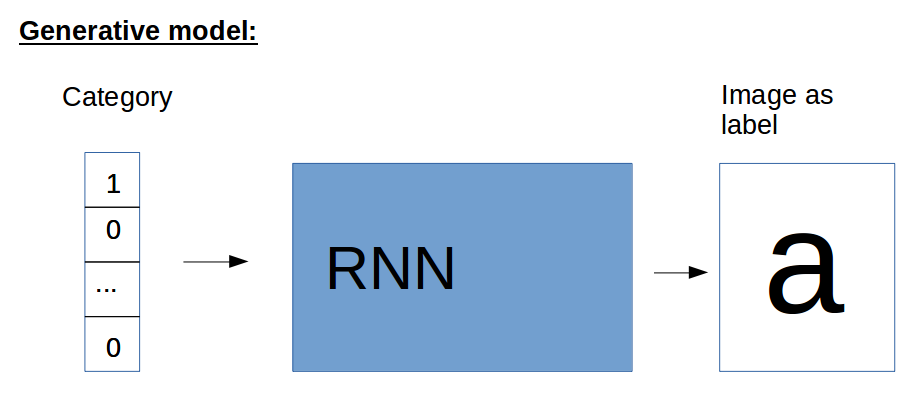
\includegraphics[width=\textwidth]{images/generative_model.png}
	\caption{Depiction of the sequence generation.}
	\label{fig:generative_model}
\end{figure}

\section{Inverse Classification}

The fully trained generative model is now used for inverse classification. Importantly, during the entire classification process the network weights are not changed. The success of the classification relies only on the concepts learned during the generative training. To classify a given target sequence, a character is generated. Since there is no prior information which character the target might be, the first generation is always performed from a uniformly distributed input vector. The resulting sequence is then compared to the sequence representing the target and an error is calculated. The gradient of the first layer of the network with respect to that error is then calculated and the uniformly distributed vector can be adapted proportional to the gradient. This process is done multiple times either until the input converges towards a static vector or the classification process is stopped after a given amount of steps. In the optimal case the input converges towards the one-hot vector representing the class of the target. Mathematically speaking, the inverse classification can be thought of as the inverse function to the generation. This implies that $f^{-1}(f(x)) = x$ if the inverse classification process works optimal, where $f(x), f^{-1}(x)$ denote the generative network and inverse classification respectively. A graphical interpretation of the process can be found in figure \ref{fig:inverse_classification}. 

\begin{figure}[!htb]
	\centering
	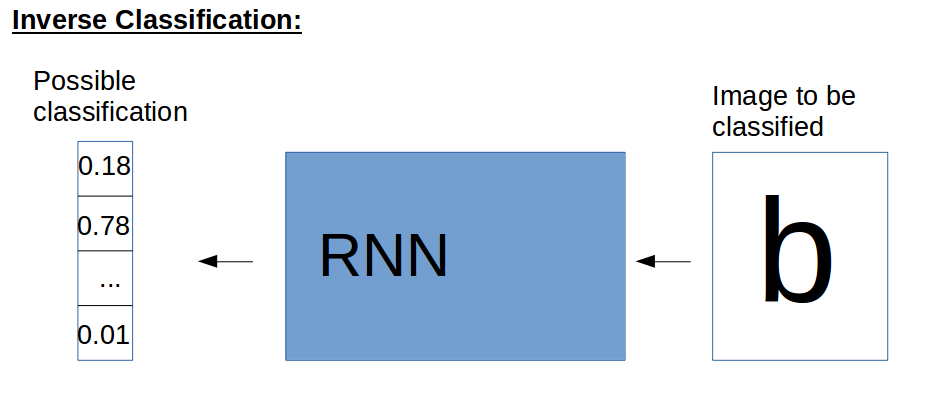
\includegraphics[width=\textwidth]{images/inverse_classification.png}
	\caption{Depiction of the inverse classification.}
	\label{fig:inverse_classification}
\end{figure}

